\section{数据库设计}\label{sec:database}
\ChapterOwner{A}{C、D}
\subsection{建模范围与数据域}
\Writing{A}{从业务事实划分身份、知识、学习世界、问答、资料、练习成长、协作、运维。区分概念模型、关系模式和物理设计。2026-11-17 目录快照有 55 个逻辑表、106 条 FK，排除分区子表和视图；定稿时重导并标实际日期。}

\subsection{教材式 ER 模型与语义}
主图精选核心学习链，包含 13 个实体、12 个菱形联系和 21 个椭圆属性。矩形为实体，菱形为联系，椭圆为属性，下划线标键，数字表示最大基数，双线表示全参与。图没有画出的字段通过核心列说明和分域字典补足。
\Writing{A}{逐段讲资料版本链、消息知识点链、作答证据链。说明消息角色 ISA 是同一消息表的分类；版本表采用全局 ID，不因有外键就认定为弱实体。主图与实现映射逐项核对。}
\begin{landscape}
\begin{figure}[p]\centering
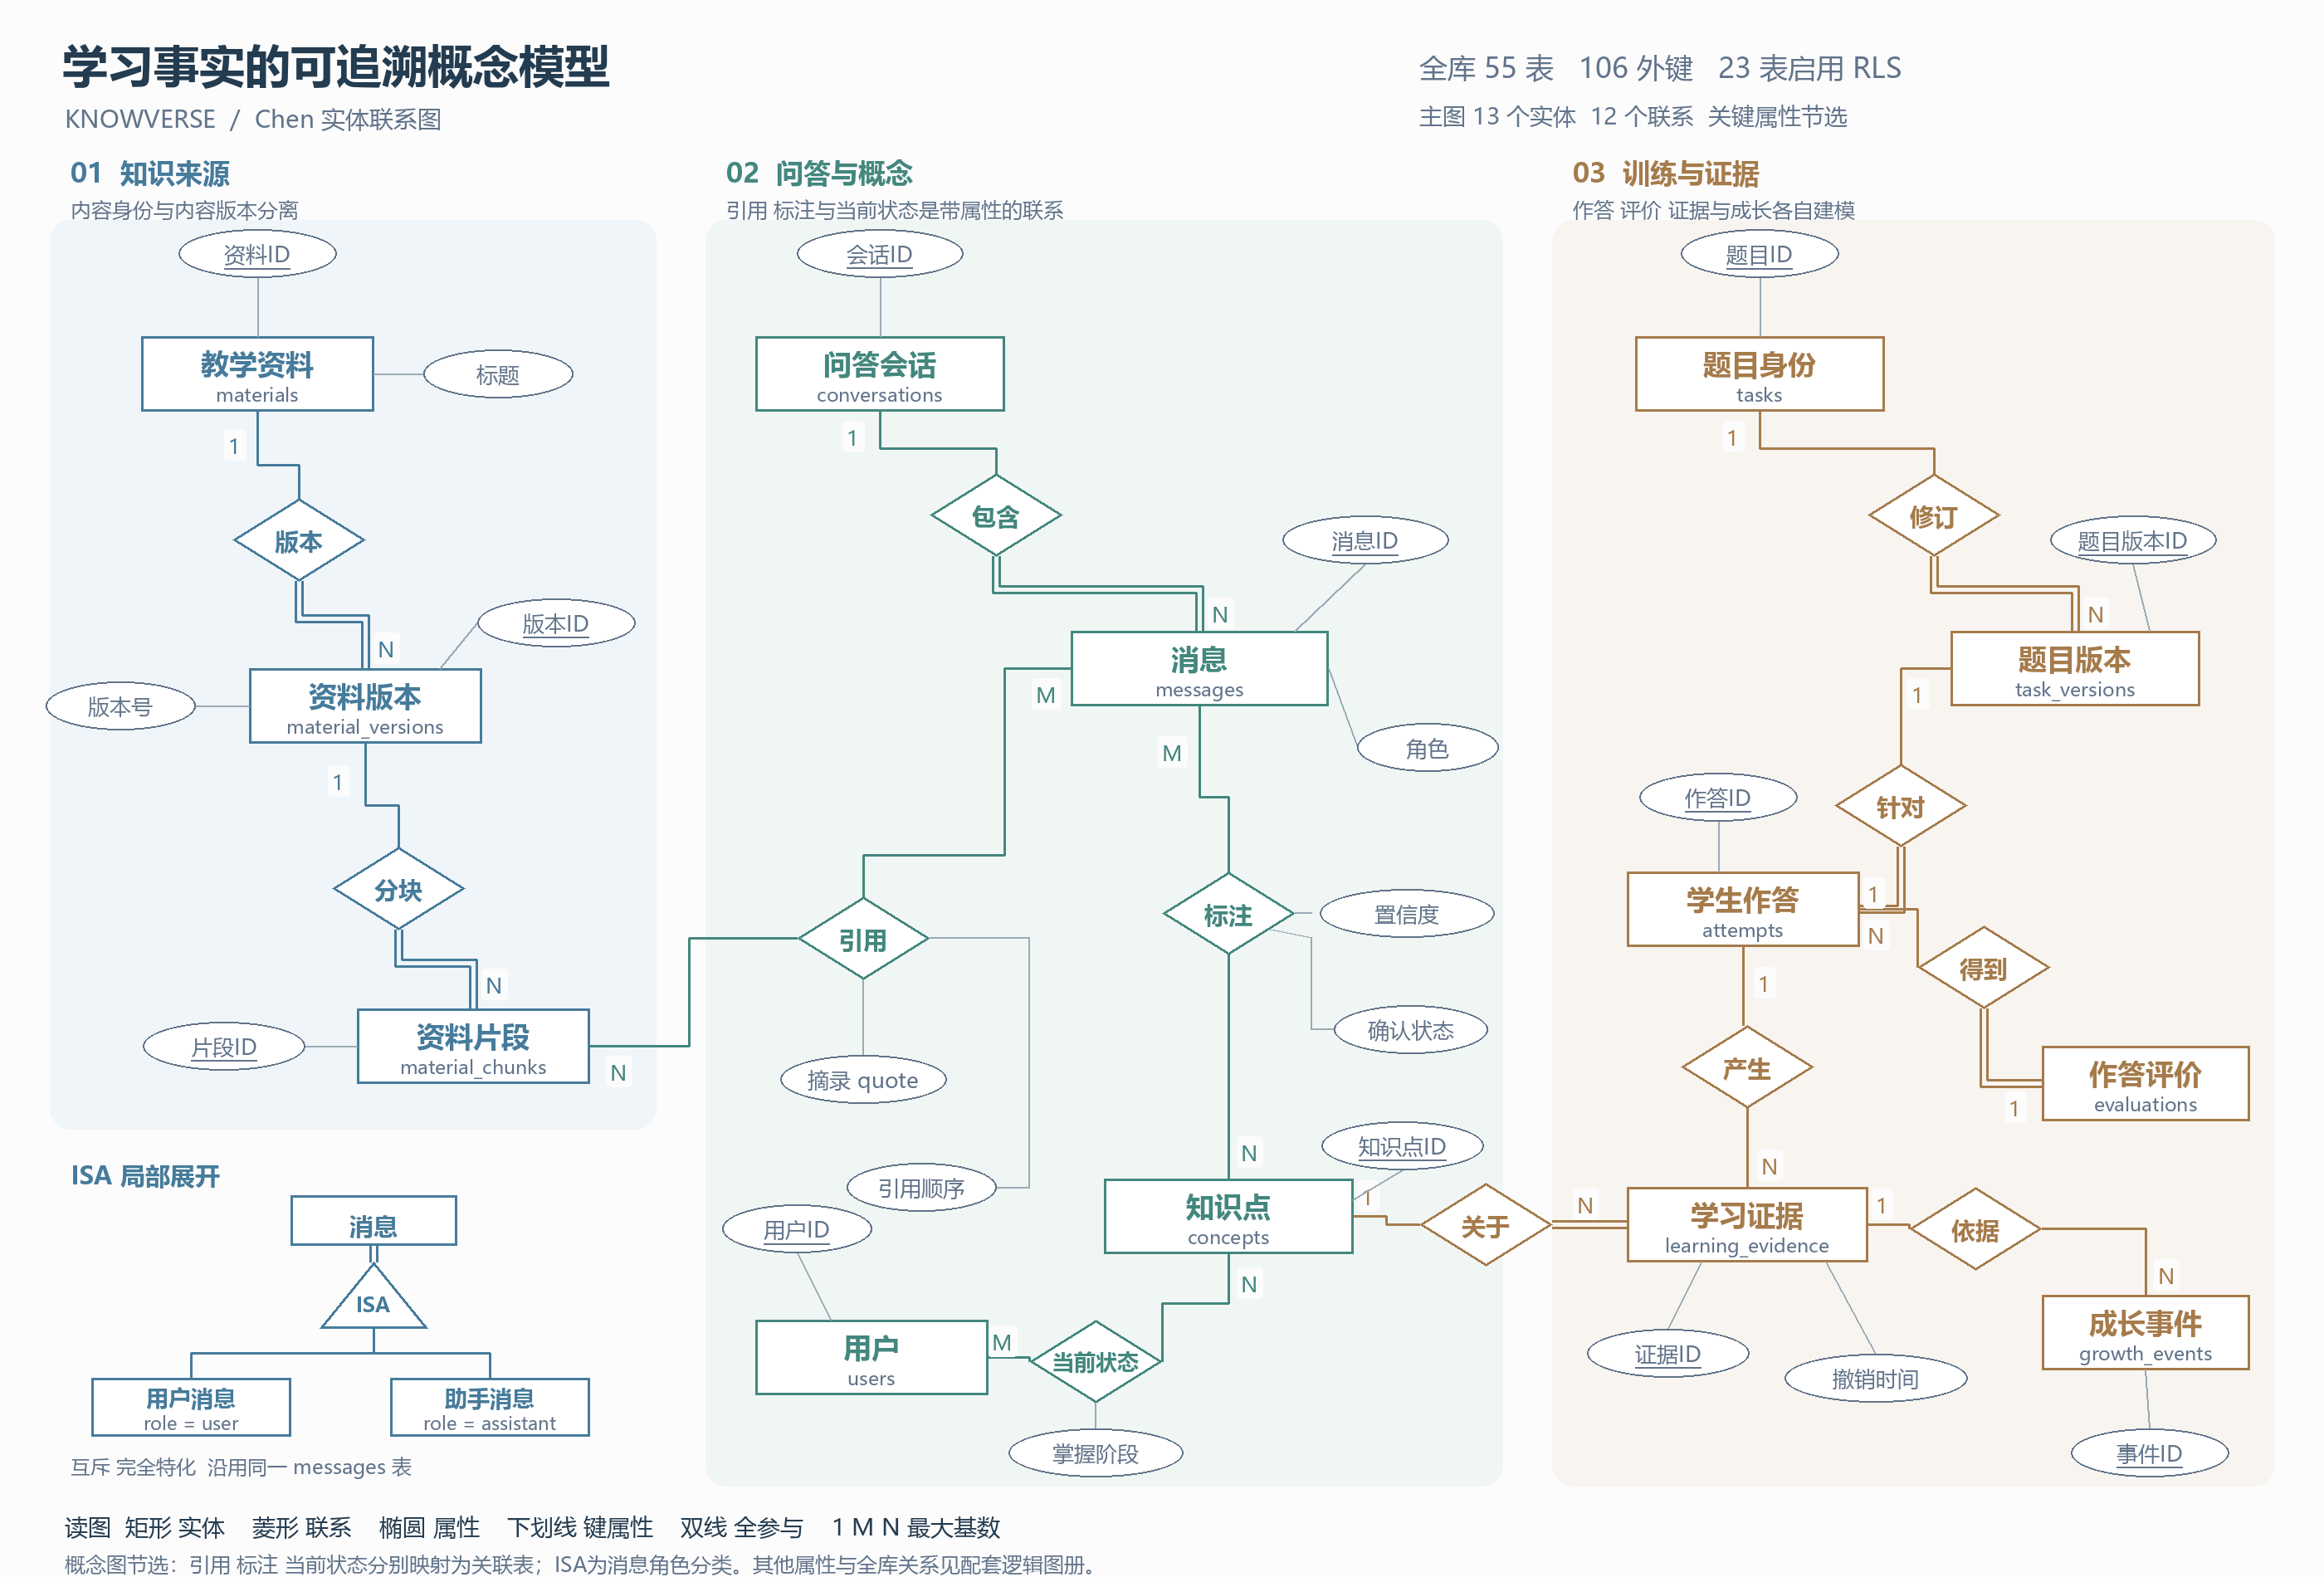
\includegraphics[width=\linewidth,height=.82\textheight,keepaspectratio]{../../er/advanced/03-learning-model.png}
\caption{实际系统核心 Chen 概念模型，属性经过精选；完整映射见图册}\label{fig:chen}
\end{figure}
\end{landscape}

\subsection{概念模型到关系模式的映射}
\Writing{A}{分别解释实体、1:N、M:N、带属性联系、自关联、ISA 如何映射。核心列至少覆盖问答标签、资料引用、练习证据三组，标类型、可空、PK/FK/UQ 和含义。}
\subsubsection{核心字段与示意数据}
以下列均来自系统目录，表中仅选关键列，非完整字典。C1、Q1、A2 等是方便讲解的符号，真实标识类型为 UUID，不能当作数据库实测记录。
\begin{table}[htbp]\centering\small
\begin{tabularx}{\linewidth}{lY}
\toprule 关系 & 精选字段及作用\\\midrule
\code{messages} & \code{id, conversation_id, user_id, seq, role, content, reply_to_id, status}：消息身份、归属、顺序、内容、回复对象与处理状态\\
\code{message_concepts} & \code{message_id, concept_id, source, status, confidence}：一条消息与一个知识点的关联及确认状态\\
\code{material_versions} & \code{id, material_id, version_no, status}：某份资料的确定版本\\
\code{material_chunks} & \code{id, version_id, ord, page_no, content}：该版本内的片段、位置与原文\\
\code{message_citations} & \code{id, message_id, chunk_id, ref_label, quote, ord}：一次回答引用哪个片段、摘录什么\\\bottomrule
\end{tabularx}
\caption{核心字段示意；类型、可空性与约束由作者补充完整}\label{tab:columns}
\end{table}
\Writing{A，C 核对}{补 Q1/A2 与片段 X1、版本 V1、资料 M1 的几行示意，展示按 chunk、version、material 外键追溯，再补作答/评价/证据/状态字段与实例。}

\subsection{候选键、函数依赖与规范化}
\subsubsection{候选键和函数依赖的业务含义}
\Writing{A}{先解释“哪些列能唯一确定一行”“某属性由谁决定”，再列 4--6 个真实关系的候选键与 FD。可空 UNIQUE、部分唯一、非最小超键单列；代理主键不代表其他依赖自动消失。}
\subsubsection{宽表异常、局部分解与无损连接}
\Writing{A}{把宽表和分解后的关系并排画在这里。用同一组用户、知识点和状态说明哪里重复、修改一条数据会影响哪些行，再给出局部无损分解的根据。}
\subsubsection{已核实结论与未证明边界}
\Writing{A，C 复核}{按最新范式复核分析版本、片段、知识点关联、引用、消息等。旧全库 46/5/4 统计已经撤回，不再宣称全库 BCNF、4NF、5NF。引用摘录由每次引用选择，不存在 \code{chunk_id} 决定 \code{quote} 的 FD。}

\subsection{受控冗余与应用便利性的权衡}
\code{messages.user_id} 与会话归属重复，对候选键 \code{(conversation_id,seq)} 存在部分依赖，严格不满足 2NF。系统保留它用于本表用户过滤，并用复合外键强制与会话一致。
\Writing{A}{再讲当前学习状态、倒排与汇总的维护、对账、读写代价。跨表可重算不是自动违反本表 3NF；少一次 JOIN 的预期不作为已经测得的收益。}

\subsection{完整性约束与业务规则}
\Writing{A}{用真实 DDL 说明 PK/FK/UNIQUE/NOT NULL/CHECK、复合与延迟约束。选引用、消息归属、本命花、先修防环、成员资格、幂等六例；解释约束、触发器、函数、应用检查各能覆盖什么。}

\subsection{查询语义与物理设计}\label{sec:query-design}
\subsubsection{用户要查什么、结果怎样组成}
\Writing{A，C 核对}{用一组问答说明关键词、时间、知识点与排序。知识点查询返回问题及其最新回答：Q1 最新 A2，旧 A1 有 K、Q1/A2 无 K，则筛 K 不能返回 Q1；问题与最新回答都命中也只出一组。}
\subsubsection{原查询与候选集合改写}
\Writing{A}{把原查询和候选集合改写并排画在这里，标出筛标签、取最新回答和去重。两侧用同一组示例行。讲清结果为什么相同，再贴必要的 SQL。实验结果放第\ref{sec:testing}章。}
\subsubsection{索引与维护成本}
\Writing{A}{把 B 树、GIN/倒排、部分索引与实际读写对应。用执行计划说明扫描次数变化，保留覆盖索引负优化案例，不泛称加索引必然更快。}

\subsection{事务、并发与失败恢复}
\Writing{A}{模型调用放事务外；前后短事务保存 pending 与回答引用。作答结算解释锁、唯一性和幂等，评价/证据/状态/事件/outbox 原子写入。并发重复提交、最后名额、中途失败各一例；outbox 原子写入不等于消费可靠性已闭环。}

\subsection{数据库安全与访问控制}
\Writing{A}{owner、\code{kv_app}、\code{kv_sandbox} 分开；事务局部身份与 RLS；甲乙用户、无上下文、池复用用非所有者验证；班级共享按成员与偏好受控。23 表 RLS 是快照覆盖信息，不代表全部表同策略或绝对安全。}

\subsection{视图、时态、审计与模式演进}
\Writing{A}{视图/物化/增量的新鲜度、审计分区、有效证据重放、迁移演进与从零建立。CDC、在线 DDL、批处理等专项择要写，详材放附录。}
\Evidence{docs/er/advanced/; docs/schema/normalization-analysis.md; docs/schema/candidate-keys.md; src/db/schema.ts; drizzle/}
